
\subsubsection{GameState}

Durante la prima sprint mi sono occupata di definire \textit{GameState}, ovvero un object che rappresenta il mezzo con cui i componenti esterni possono interfacciarsi con gli elementi che costituiscono la logica di gioco in modo da esporre all'esterno solamente le informazioni che effettivamente sono necessarie all'interazione con essa.
    \begin{figure}[H]\centering
      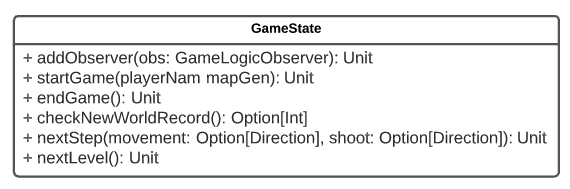
\includegraphics[width=12cm]{res/GameState-uml.png}
      \caption{Metodi pubblici in GameState}
      \label{gameState}
    \end{figure}


\subsubsection{updateMap}

Successivamente mi sono occupata della gestione della notifica di movimento del player da parte del controller. In un primo momento, la notifica di tale movimento era processata attraverso un semplice spostamento del personaggio da una posizione a quella vicina nella direzione in cui era stato richiesto lo spostamento.


\subsubsection{Collectibles}

Ho introdotto le due tipologie di oggetti collezionabili e la loro gestione. La prima permette al giocatore di recuperare una vita nel caso in cui non abbia già il numero massimo di vite possibili, la seconda incrementa il punteggio della specifica partita.
Per differenziare le diverse modalità di gioco, all'interno della classe di utility \textit{Difficulty} ho inserito un parametro che permette di generare un diverso numero di bonus in base alla difficoltà scelta.
Le due case class di bonus estendono un'unica sealed trait \textit{Collectible} perciò non potranno essere inseriti nuovi bonus esternamente se non andando ad introdurli all'interno dello stesso sorgente.
In questo caso, mi sono occupata anche della parte grafica dei diversi collectibles. 

\subsubsection{Hero}

Le caratteristiche principali del personaggio riguardano le vite a disposizione che verranno incrementate o decrementate in base alle sue azioni e lo score ottenuto attraverso l'uccisione di un nemico o raccogliendo un bonus che ha come effetto un'incremento del punteggio.

\subsubsection{Enemy}

L'entità relativa ai nemici è caratterizzata da un movimento randomico che permette ad ognuno di essi di spostarsi. Inoltre, anch'essi, come l'hero, vengono generati con un totale di cinque vite che verranno poi decrementate ad ogni colpo sparato dal personaggio.

\subsubsection{Door}
In collaborazione con L
orenzo Chiana, mi sono occupata della terminazione di un livello e la generazione di quello successivo. In particolare, ho sviluppato la parte relativa alla fine del livello che avviene individuando l'assenza di nemici e che provoca creazione in una posizione randomica della \textit{Door} che permette al personaggio di passare al livello successivo. 

Una volta che la posizione del player corrisponde con quella della porta di uscita verrà creata una nuova mappa con la porta d'ingresso nella posizione esattamente opposta rispetto a quella da cui l'hero era uscito al livello precedente.

\begin{figure}[H]\centering
  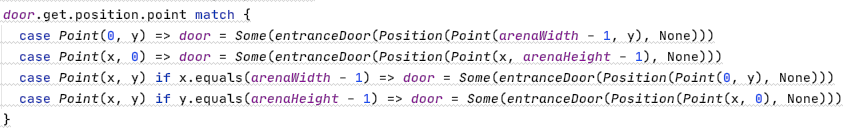
\includegraphics[width=15cm]{res/createOppositeDoor.png}
  \caption{Creazione della porta d'ingresso nella posizione opposta a quella di uscita nel livello precedente.}
  \label{gameState}
\end{figure}

All'inizio di una partita, viene creata una porta fittizia, anch'essa in maniera randomica, in cui viene posizionato il giocatore.
Il giocatore, finchè si trova all'intero della porta d'ingresso, non può sparare ai nemici.

\begin{figure}[H]\centering
  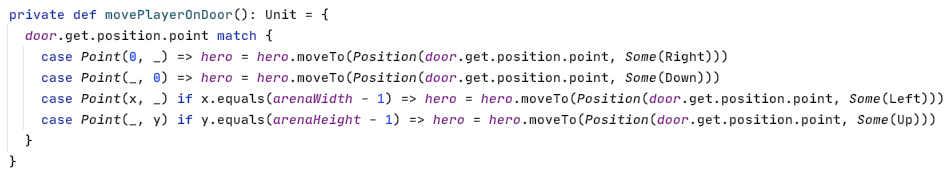
\includegraphics[width=15cm]{res/movePlayerOnDoor.png}
  \caption{Posizionamento del giocatore all'interno della porta d'ingresso.}
  \label{gameState}
\end{figure}


